\documentclass[11pt, oneside]{article}   	
\usepackage{geometry}  
\usepackage{array}              		
\geometry{letterpaper}                   		           		
\usepackage[parfill]{parskip}    		
\usepackage{graphicx}												
\usepackage{amssymb}


\title{Advanced Programming Assessed Exercise Report}
\author{Paul McHard - 2085227M}
\date{\today}						

\begin{document}
\maketitle
\subsection*{Assumptions}
\begin{itemize}
\item{It is assumed that traffic will only move one way along a given row or column. In testing the contrary would cause deadlocks.}
\item{It is assumed that all cars are of unit size and occupy only one block, and there is no expectation to model larger vehicles.}
\item{It is assumed that cars do not change direction as they move through the grid.}
\item{It is assumed that writing to a .txt file is appropriate output for the statistics report.}
\item{It is assumed that it is desirable for a user to be presented stats information with seconds as the base unit not milliseconds.}
\end{itemize}

\subsection*{Class Design}
This section includes the UML Class Diagram for the system and then briefly discusses each class and its methods.
\newpage

\begin{figure}[h!]
\centering
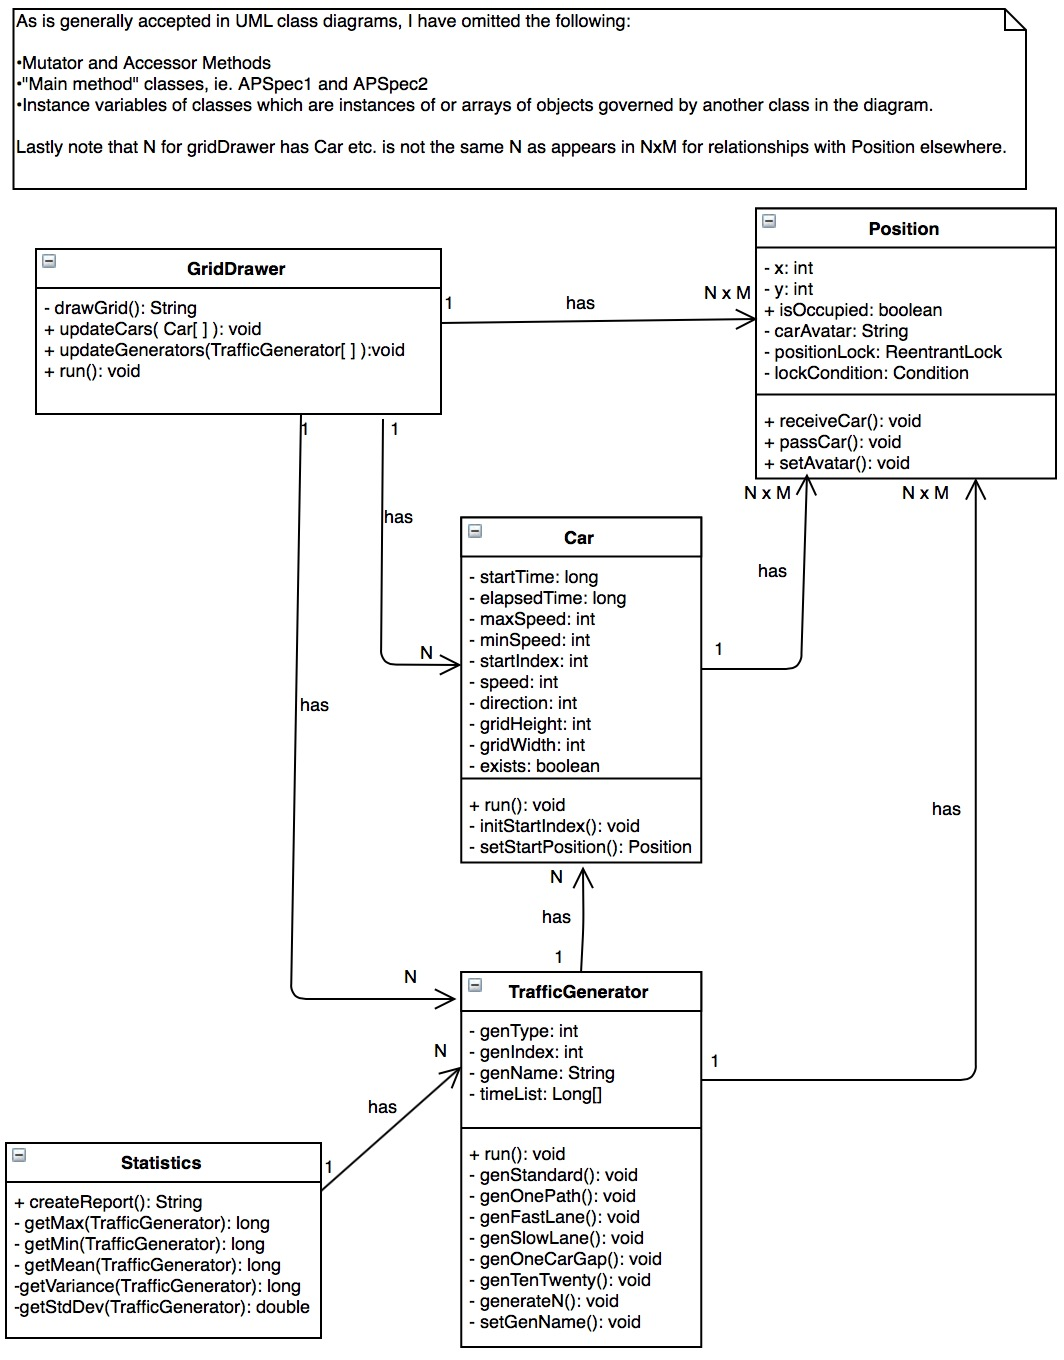
\includegraphics[width=0.9\textwidth]{APAEUML}
\caption{UML Class Diagram.}
\end{figure}

\subsubsection*{Car}
\texttt{initStartIndex()}: randomises start Index within the bounds of grid Height or grid Width respectively based on direction of cars travel.

\texttt{setStartPosition()}: Determines which edge the car should start on based on the direction it will travel. The car is put into the (\texttt{startIndex})th position along said edge.

\texttt{run()}: Called by the the Thread starting. Handles calculating what the next position the car should go to is, handles motion of the car to that position and leaving position before and repeating until the car reaches its last position, at which point it removes the car and calculates the elapsed time.

\subsubsection*{Position}
\texttt{receiveCar()}: Handles receiving a car into itself and locking and lock conditions involved.

\texttt{passCar()}: Handles passing a car out of itself and locking involved.

\texttt{setAvatar()}:Sets the `Avatar' for the car occupying the position (which arrow type is shown in the grid) based on direction value of occupant car.

\subsubsection*{GridDrawer}
\texttt{drawGrid()}: `draws' the output grid as a String based on occupancy of positions at that exact instant. 

\texttt{updateCars()}: Allows the array of cars which are rendered to be updated, necessary for spec 1.

\texttt{updateGenerators()}: Allows the set of traffic generators fed into the GridDrawer, and therefore the array of cars being rendered, to be updated. Useful but not necessary for spec 2.

\texttt{run()}: Called by Thread being started. Handles the ``refreshing" of the grid every 20ms. Repeats for 2000 times as specified calling drawGrid and sleeping for 20ms.

\subsubsection*{TrafficGenerator}
\texttt{run()}: Called by the Thread starting, switch case calls one of the generator types which is specified as a input variable in the constructor.

\texttt{genStandard()}: Loops through the array of cars three times. First loop makes and starts a Thread for the car. The second loop uses the Thread's join function to wait for all them to conclude. The last loop generates an array of the elapsed times of all cars.

\texttt{genOnePath()}: Sets all cars to have the same inputted start index then calls \texttt{genStandard()}.

\texttt{genFastLane()}: Similar to \texttt{genOnePath()}, but additionally sets all cars in the generator to have maximised speed.

\texttt{genSlowLane()}: Similar to \texttt{genOnePath()}, but additionally sets all cars in the generator to have minimised speed.

\texttt{genOneCarGap()}: Sets all cars to same track, as per \texttt{genOnePath()}, then runs similar to \texttt{genStandard()}, but sleeps for the most recent car's `speed' between starting each cars thread, effectively taking a pause equivalent to the most recent car.

\texttt{genTenTwenty()}: generates the pattern through the entire grid to match the specific example given in the second bullet of spec 2.

\texttt{generateN()}: there are multiple overridden versions of this method. It creates the array of N car objects for the generator and has the ability to dictate the direction or both direction and speed.

\subsubsection*{Statistics}
\texttt{createReport()}: creates a String output which displays stats for time taken for each Traffic Generator.

\texttt{getMax()}: calculates Maximum elapsed time in generator.

\texttt{getMin()}: calculates Minimum elapsed time in generator.

\texttt{getMean()}: calculates Mean elapsed time in generator.

\texttt{getVariance()}: calculates Variance in elapsed times in generator.

\texttt{getStdDev()}: calculates Standard Deviations of elapsed times in generator.

\subsection*{Testing}
The following tests were performed to assess the system's performance. 

\begin{center}
\begin{tabular}{ | m{8cm} | m{8cm} | } 
 \hline
Test & Result \\ 
 \hline
 1.Test if program can handle a grid of length 0 in either direction. & Program fails and throws an error. \\ 
 \hline
 2.Test if program can handle an exceedingly large grid size. Tested with 500x500.  & Difficult to view on console but program is capable of output. \\ 
 \hline
 3.Test exceedingly highly populated simulation. Tested with 500 cars in 10x20 grid. & Simulation ends with cars in array because gridDrawer ends due to 2000 repeat limit. System successfully renders simulation for duration. \\
 \hline
 4. Test that Reentrant Lock and Lock Condition are functioning properly with 1x1 grid, one car moving east, one moving south. & Successfully simulates system, Space is occupied by one car first, which is cleared, and then the other enters an is cleared. \\
\hline
5. Test that two cars on same row moving in opposite directions will cause a deadlock. & As expected the system deadlocks and neither move. Evidence in Figure 1. \\
 \hline
6. Test that two cars on same column moving in opposite directions will cause a deadlock & Same result as above.\\
 \hline
7.Test that four cars can be in deadlock if they arrive in a square formation simultaneously. & Expected deadlock demonstrated. \\
 \hline
8. Test that system will not allow traffic generator to dictate startIndex of cars if index is specified which is out of bounds. & System defaults to random distribution with genStandard(). \\
 \hline
9. Test that system will default to genStandard() if a genType which is out of bounds is specified. & Result is as expected in test. \\
 \hline
10. Test that Statistics outputs successfully at end of spec 2 for multiple generators. & Result is as expected. \\
  \hline
\end{tabular}
\end{center}
 
 \subsubsection*{Deficiencies}
 One deficiency that is to be noted is that in highly populated simulations, horizontally moving cars in the top and bottom row will on occasion render with the incorrect arrow and be shown with a vertical moving arrow, either north or south. Movement is still normal and there is no issue of lock breaking but wrong symbol is displayed. This is an error I have not been able to rectify within the timeframe of the project.


\subsection*{Questions}
\begin{enumerate}
\item{One extension that my model in its current state could not handle would be a system which desires the car to be able to change direction, such as simulating turning corners, while the car exists within the grid. It could be possible with a very particular Traffic Generator perhaps, but I think this would still require a redesign of how the Car processes its movement. The Position and Grid Drawer classes could be used unchanged in this extension but I am confident the Car object would need a major redesign to cope.}
\item{One extension that I feel my model could handle effectively would be the ability to handle addition of extra generators while others are already running. The GridDrawer class has an updateGenerators() method already, which just needs to be passed the most up to date array of traffic generators in use and there would be no problems and it will update its array of Cars to include the newly generated instances.}
\item{In Theory, I believe this extension could be implemented in my system without major changes required to the Car, Position or Statistics Classes. A car will still have a path to follow and Position will still be a point in the array which passes and receives cars and handles locking. At present, both spec 1 and spec 2 in my solution a simple 2D array of position objects to represent the NxM grid. I believe that the first step to the solution would be implementing a new Intersection class which would essentially be the NxM array of positions, and would also handle how each instance of itself are related, ie. which `streets' of intersection A lead to which `streets' of intersection B. Car would perhaps need minor adjustments to handle moving from one intersection to another, but I would also consider that this problem could be solved by TrafficGenerators, which would need to be altered and developed upon to channel cars through the connecting intersections. The GridDrawer class would also need updated to draw a larger map featuring multiple intersections and do so in a way that was visually pleasing, but this part of the solution would be reasonably trivial compared to the other required changes I've discussed.

 Referring back to my answer to question 1, I would still have the issue that cars would only be able to move in one direction through the entire `city', which is not a very natural or realistic model. If it was desired and with development time permitting, were this a real-life project in a working environment, I would aim to implement a solution to that problem simultaneously, and allow cars to move through the city with the ability to turn corners.}
\item{I tried to approach the task with a reasonable amount of preparation and planning before beginning to code, and endeavoured to implement MVC architecture in the system. For this reason I am proud of the solution I have presented which is based around relatively simple and cohesive classes in the form of the Car and Position classes. I designed and implemented these classes with a clear vision of what they needed to do, and I feel this is reflected in their respective cohesiveness within the model. I did however make the mistake of designing to meet spec 1 only, and as a result my extension to meet spec 2 is not as clean and cohesive. If I were going back and restarting I would redesign the TrafficGenerator class properly and include a `standard' or `randomised' Traffic Generator within spec 1. This level of forward thinking might have made spec 2 better integrated with spec 1, and could have allowed for more fluid extension beyond the current model.}
\end{enumerate}
\end{document}  